\chapter{Complementary Results}
\label{Complementary_Results}

\section{Changing the vortices' topological charge $\ell$}

The following set of figures shows regular and perfect vortices with topological charge $\ell = 6$ propagated through $z = 1000$ [mm], with their fundamental arguments unchanged. This is, $sigma = 100$ for the regular vortex and $Rpx = 764$ [px] and $N = 40$ for the perfect vortex.

\begin{figure}[htbp]
    \centering
    \begin{subfigure}[b]{0.45\textwidth}
        \centering
        \includegraphics[width=\textwidth]{images/Appendices/Additional_Results/Topological_Charge/per_6_r0.png}
        \caption{Regular vortex.}
    \end{subfigure}
    \hfill
    \begin{subfigure}[b]{0.45\textwidth}
        \centering
        \includegraphics[width=\textwidth]{images/Appendices/Additional_Results/Topological_Charge/per_6_r0.png}
        \caption{Perfect vortex.}
    \end{subfigure}
    \caption{Unobstructed vortices of state $\ell = 6$.}
    \label{fig:Vortices_L=6_r=0}
\end{figure}

\begin{figure}[htbp]
    \centering
    \begin{subfigure}[b]{0.45\textwidth}
        \centering
        \includegraphics[width=\textwidth]{images/Appendices/Additional_Results/Topological_Charge/reg_6_r30.png}
        \caption{Regular vortex.}
    \end{subfigure}
    \hfill
    \begin{subfigure}[b]{0.45\textwidth}
        \centering
        \includegraphics[width=\textwidth]{images/Appendices/Additional_Results/Topological_Charge/per_6_r30.png}
        \caption{Perfect vortex.}
    \end{subfigure}
    \caption{Vortices of state $\ell = 6$ with obstruction radius $r=30$ [px].}
    \label{fig:Vortices_L=6_r=30}
\end{figure}

\begin{figure}[htbp]
    \centering
    \begin{subfigure}[b]{0.45\textwidth}
        \centering
        \includegraphics[width=\textwidth]{images/Appendices/Additional_Results/Topological_Charge/reg_6_r50.png}
        \caption{Regular vortex.}
    \end{subfigure}
    \hfill
    \begin{subfigure}[b]{0.45\textwidth}
        \centering
        \includegraphics[width=\textwidth]{images/Appendices/Additional_Results/Topological_Charge/per_6_r50.png}
        \caption{Perfect vortex.}
    \end{subfigure}
    \caption{Vortices of state $\ell = 6$ with obstruction radius $r=50$ [px].}
    \label{fig:Vortices_L=6_r=50}
\end{figure}

\begin{figure}[htbp]
    \centering
    \begin{subfigure}[b]{0.45\textwidth}
        \centering
        \includegraphics[width=\textwidth]{images/Appendices/Additional_Results/Topological_Charge/reg_6_r70.png}
        \caption{Regular vortex.}
    \end{subfigure}
    \hfill
    \begin{subfigure}[b]{0.45\textwidth}
        \centering
        \includegraphics[width=\textwidth]{images/Appendices/Additional_Results/Topological_Charge/per_6_r70.png}
        \caption{Perfect vortex.}
    \end{subfigure}
    \caption{Vortices of state $\ell = 6$ with obstruction radius $r=70$ [px].}
    \label{fig:Vortices_L=6_r=70}
\end{figure}

\begin{figure}[htbp]
    \centering
    \begin{subfigure}[b]{0.45\textwidth}
        \centering
        \includegraphics[width=\textwidth]{images/Appendices/Additional_Results/Topological_Charge/reg_6_r100.png}
        \caption{Regular vortex.}
    \end{subfigure}
    \hfill
    \begin{subfigure}[b]{0.45\textwidth}
        \centering
        \includegraphics[width=\textwidth]{images/Appendices/Additional_Results/Topological_Charge/per_6_r100.png}
        \caption{Perfect vortex.}
    \end{subfigure}
    \caption{Vortices of state $\ell = 6$ with obstruction radius $r=100$ [px].}
    \label{fig:Vortices_L=6_r=100}
\end{figure}

\newpage
\section{Changing perfect vortices' fundamental parameters}
\subsection{Changing regular vortices' Gaussian size}

The following set of figures shows regular vortices of state $\ell = 10$ and Gaussian's standard deviation $\sigma = 150$ propagated through $z = 1000$ [mm] along with varying obstruction radii. This variation in $\sigma$ means that the Gaussian of the real field that is propagated along the regular vortex's phase mask is larger than the default value $\sigma = 100$, as it can be seen in figure (\ref{fig:2D_Gaussian_sigmas}). 

\begin{figure}[htbp]
    \centering
    \begin{subfigure}[b]{0.45\textwidth}
        \centering
        \includegraphics[width=\textwidth]{images/Appendices/Additional_Results/Sigma_150/sigma=100.png}
        \caption{$\sigma = 100$.}
    \end{subfigure}
    \hfill
    \begin{subfigure}[b]{0.45\textwidth}
        \centering
        \includegraphics[width=\textwidth]{images/Appendices/Additional_Results/Sigma_150/sigma=150.png}
        \caption{$\sigma = 150$.}
    \end{subfigure}
    \caption{Comparison between two pure 2D Gaussian beams with different standard deviations.}
    \label{fig:2D_Gaussian_sigmas}
\end{figure}

\begin{figure}[htbp]
    \centering
    \begin{subfigure}[b]{0.45\textwidth}
        \centering
        \includegraphics[width=\textwidth]{images/Appendices/Additional_Results/Sigma_150/unobs_sigma100.png}
        \caption{$\sigma = 100$.}
    \end{subfigure}
    \hfill
    \begin{subfigure}[b]{0.45\textwidth}
        \centering
        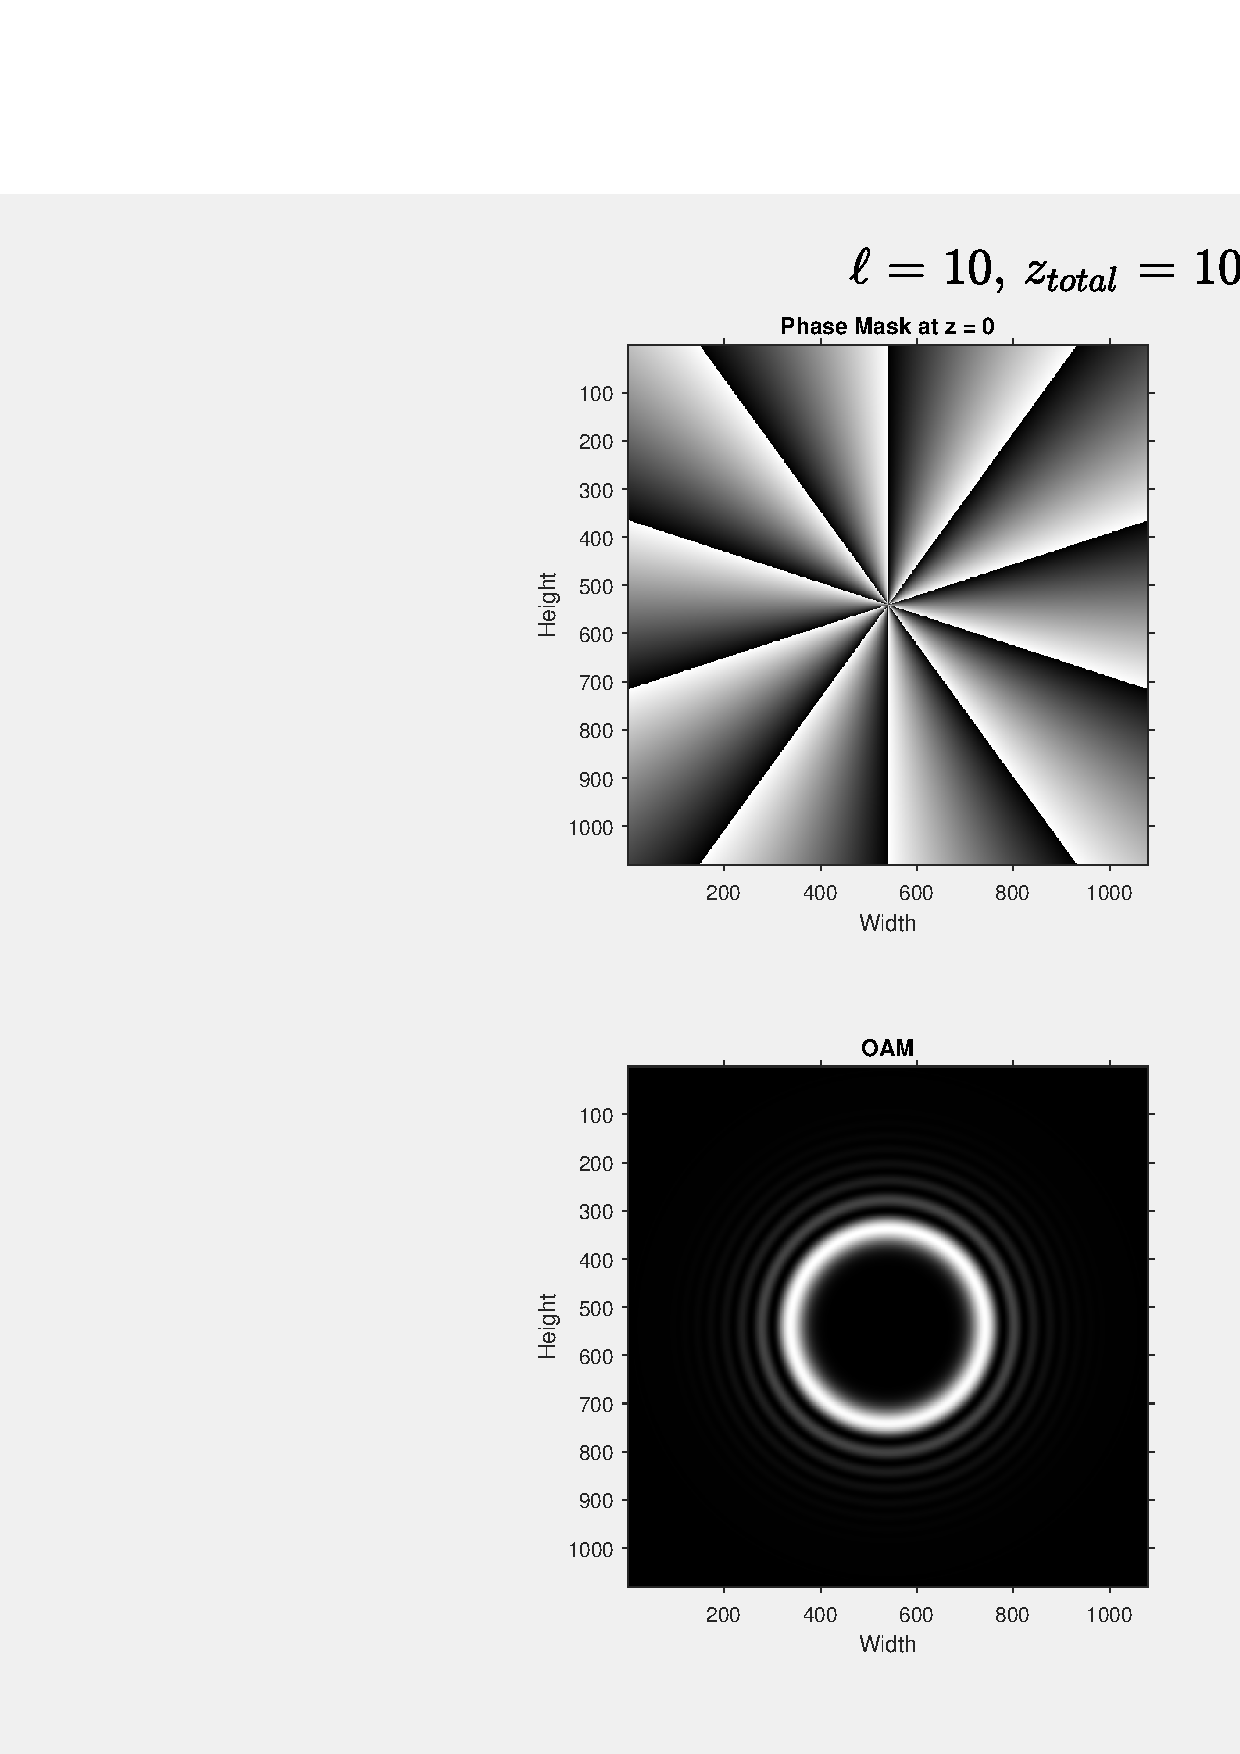
\includegraphics[width=\textwidth]{images/Appendices/Additional_Results/Sigma_150/type=0_r=0_zi=0_zf=1000.png}
        \caption{$\sigma = 150$.}
    \end{subfigure}
    \caption{Comparison between two unobstructed regular vortices with different standard deviations. Notice how a larger sigma can help further distinguish the beam's surrounding rings.}
    \label{fig:reg_sigma100-vs-sigma150}
\end{figure}

\begin{figure}[htbp]
    \centering
    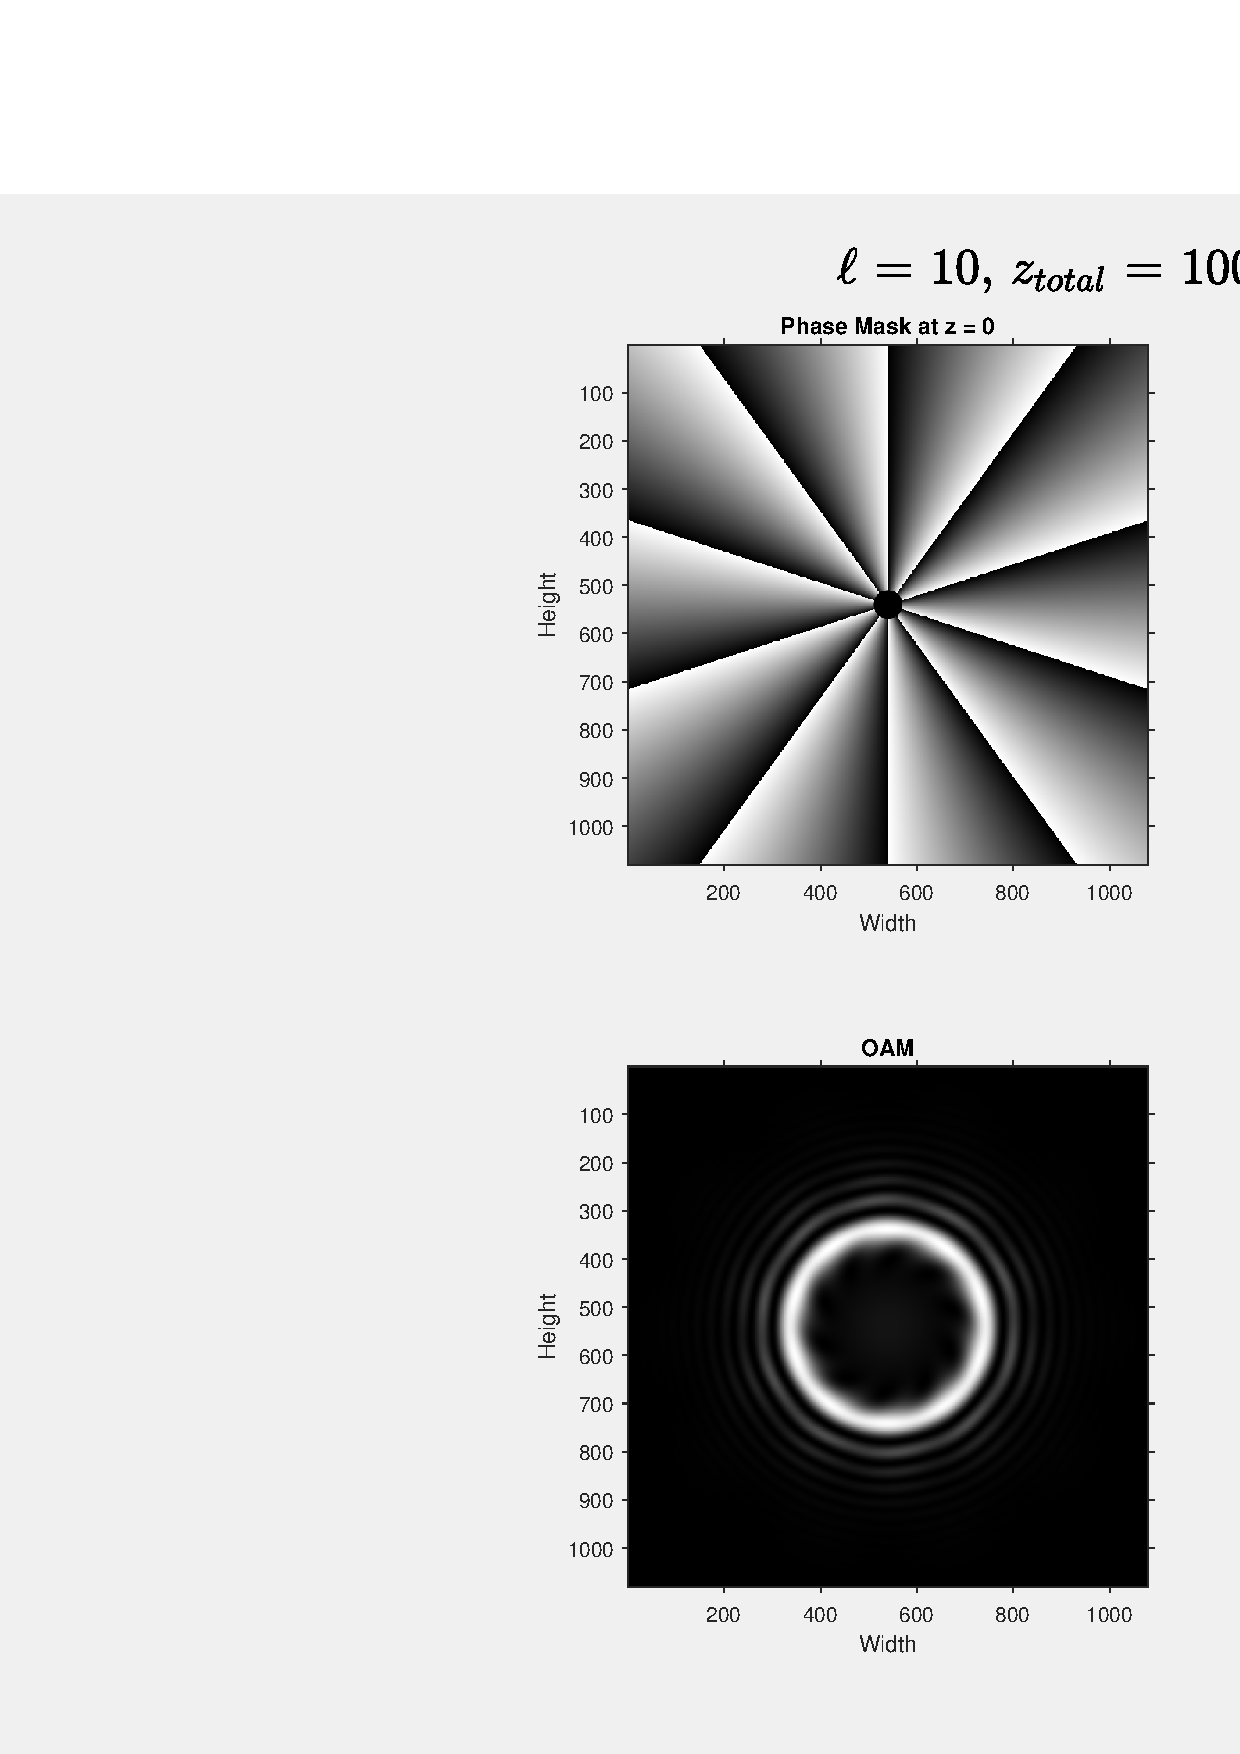
\includegraphics[width=12cm]{images/Appendices/Additional_Results/Sigma_150/type=0_r=30_zi=0_zf=1000.png}
    \caption{Regular vortex with $\sigma = 150$ and obstruction size $r=30$ [px].}
    \label{fig:reg_sig150_r=30}
\end{figure}

\begin{figure}[htbp]
    \centering
    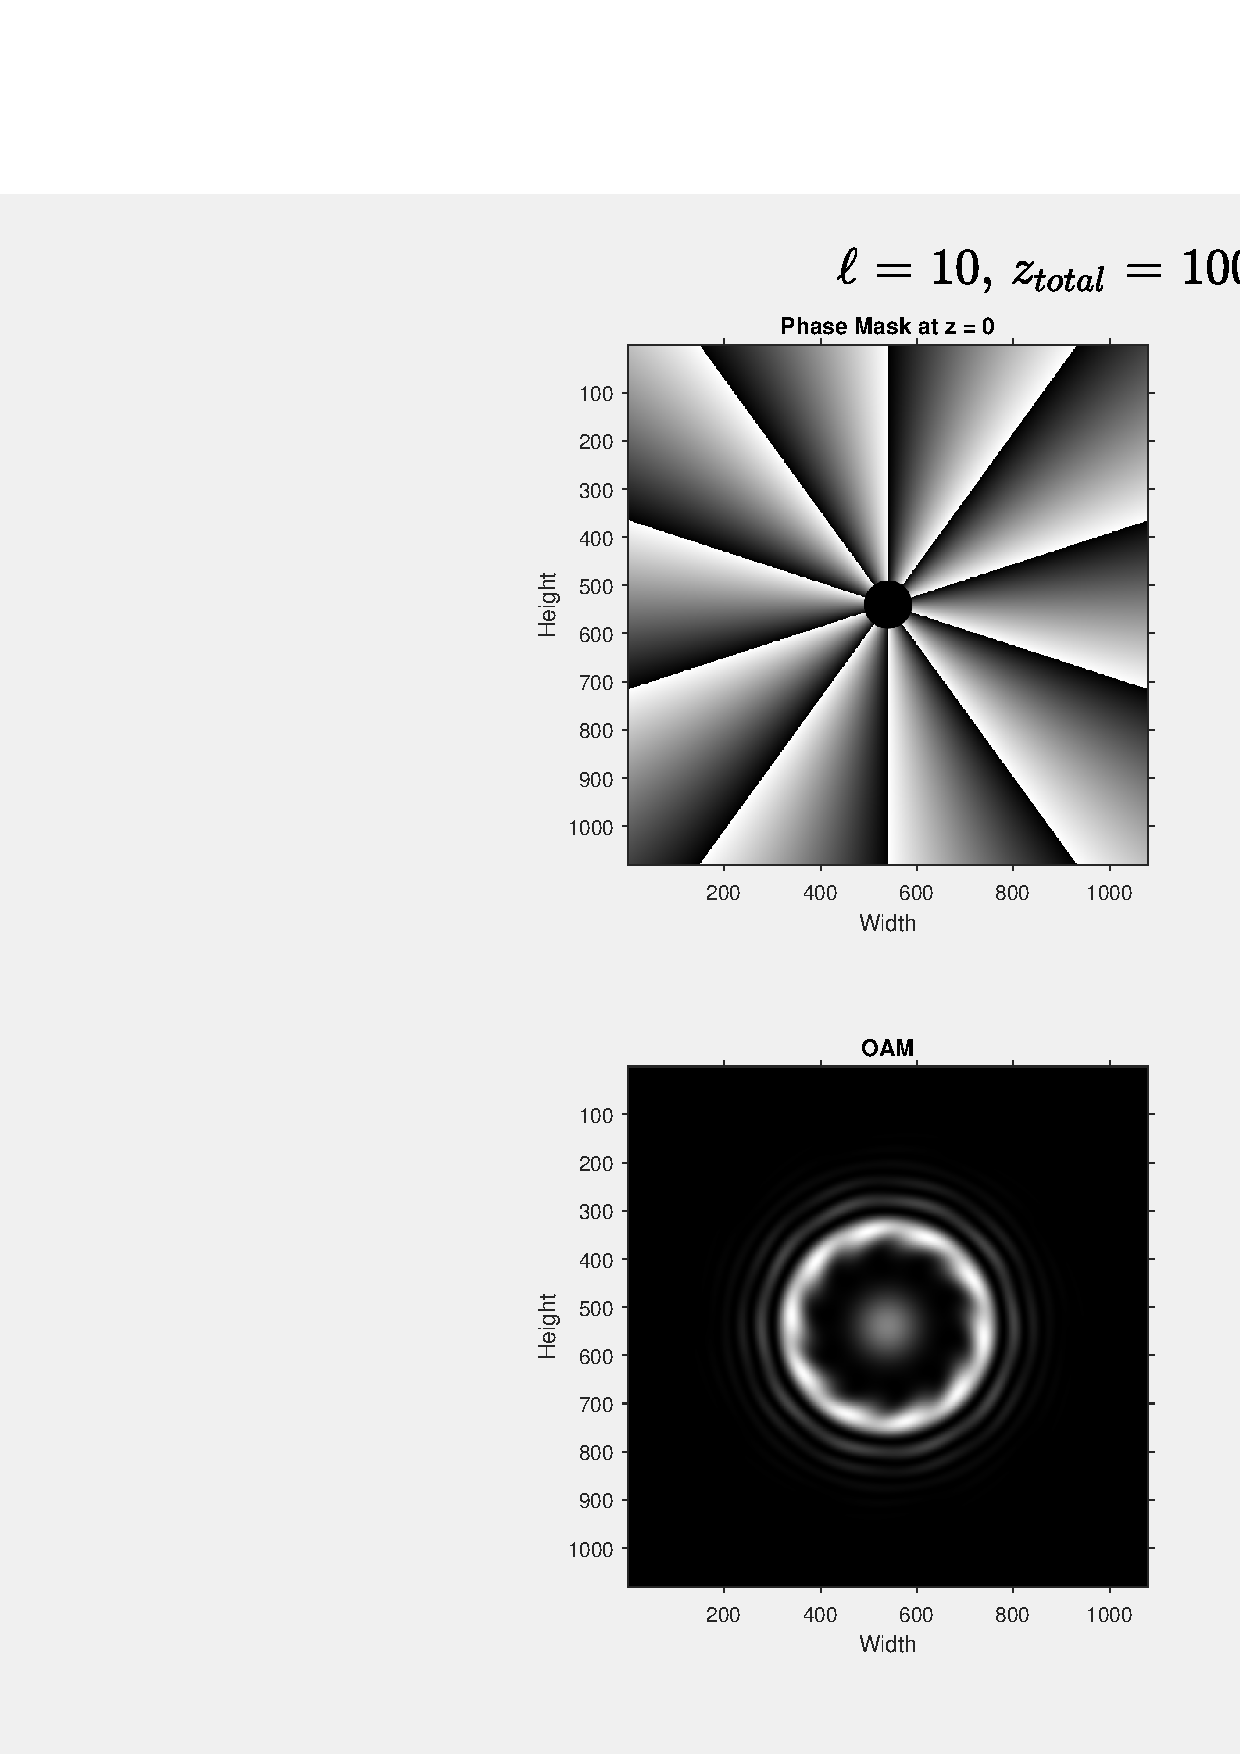
\includegraphics[width=12cm]{images/Appendices/Additional_Results/Sigma_150/type=0_r=50_zi=0_zf=1000.png}
    \caption{Regular vortex with $\sigma = 150$ and obstruction size $r=50$ [px].}
    \label{fig:reg_sig150_r=50}
\end{figure}

\begin{figure}[htbp]
    \centering
    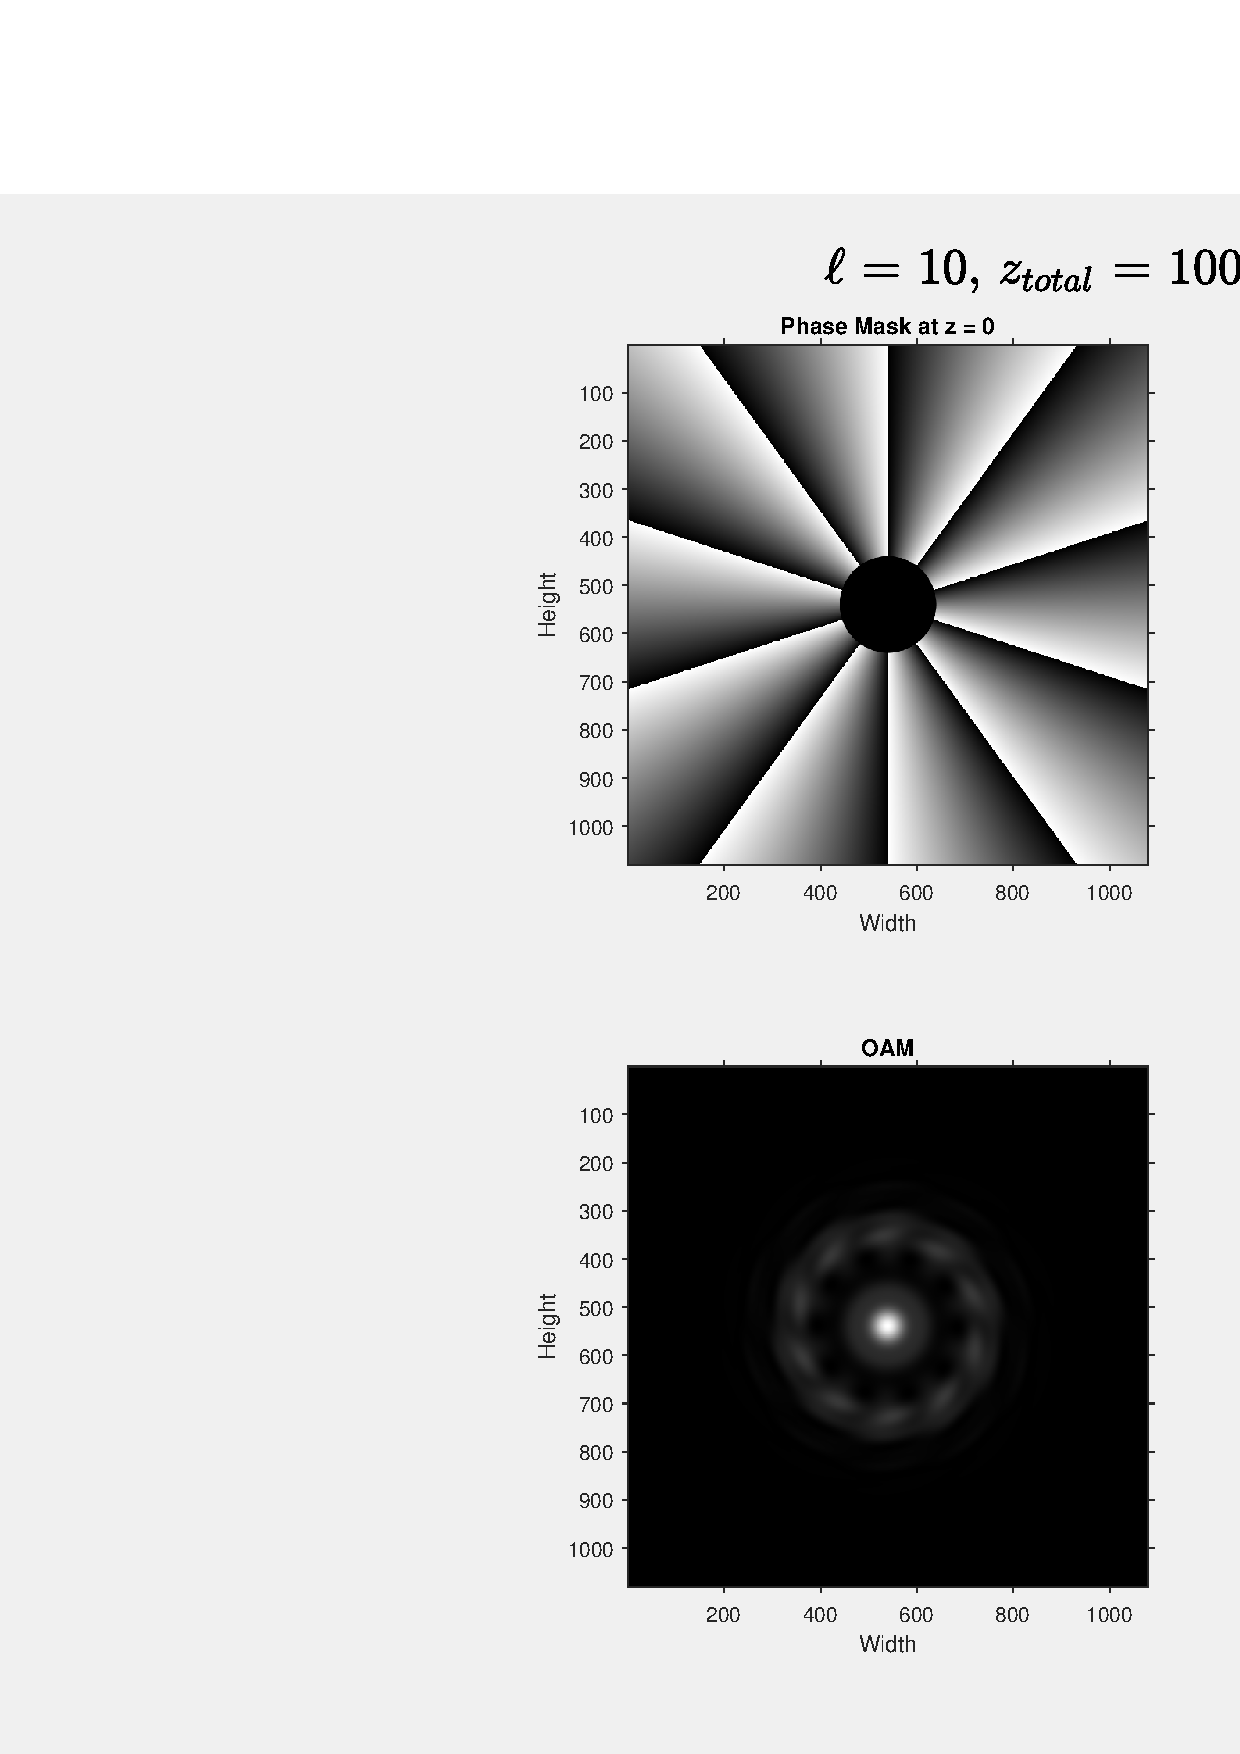
\includegraphics[width=12cm]{images/Appendices/Additional_Results/Sigma_150/type=0_r=100_zi=0_zf=1000.png}
    \caption{Regular vortex with $\sigma = 150$ and obstruction size $r=100$ [px].}
    \label{fig:reg_sig150_r=100}
\end{figure}

\newpage
\subsection{Changing perfect vortices' aperture and number of rings}
The following set of figures show perfect vortices of state $\ell = 10$ made with an aperture of $Rpx = 500$ [px] and number of rings $N = 60$. The first figure is propagated through $z = 1000$ [mm] and it clearly shows that altering the fundamental parameters distorts the vortex in a negative ways, if the propagation distance remains the same.

\begin{figure}[htbp]
    \centering
    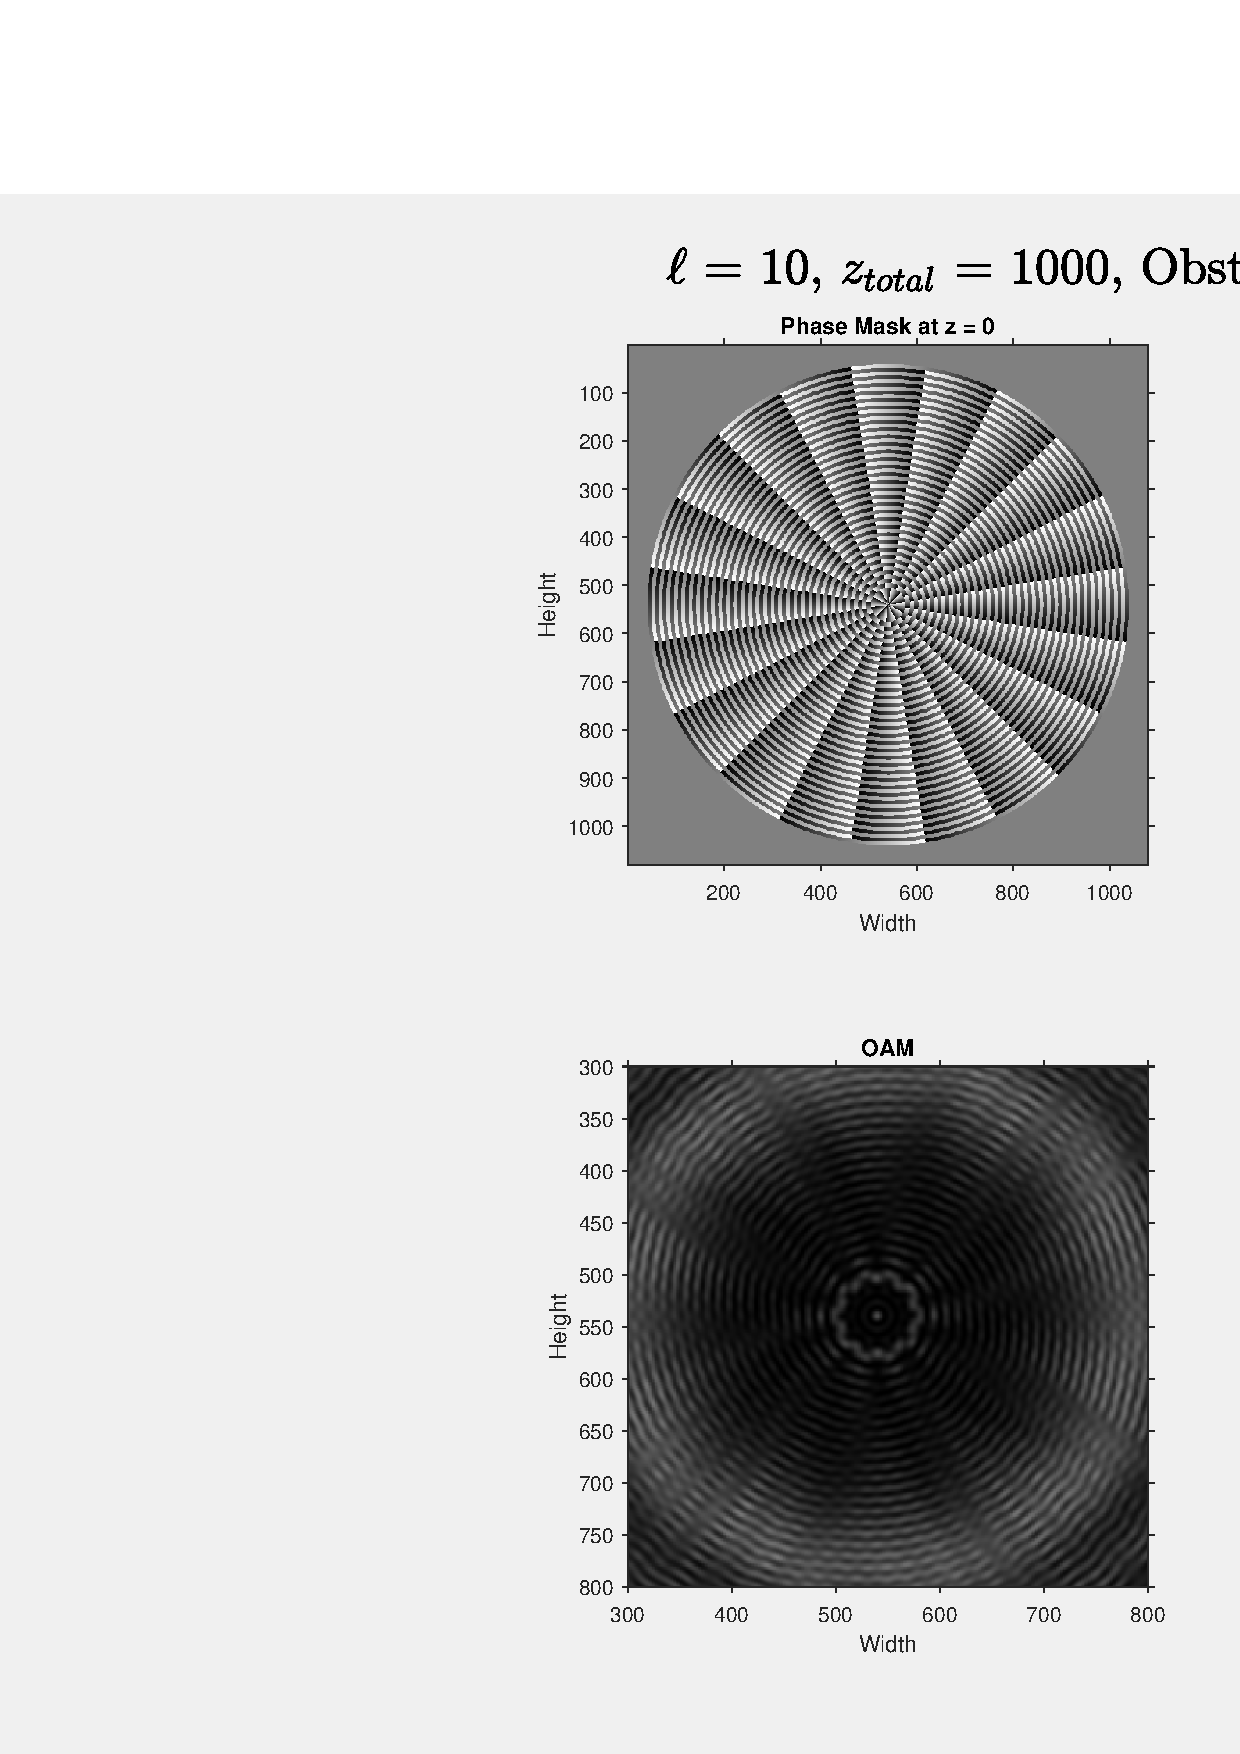
\includegraphics[width=12cm]{images/Appendices/Additional_Results/Rpx500_N60/type=1_r=0_zi=0_zf=1000.png}
    \caption{Unobstructed perfect vortex with $Rpx = 500$ [px], $N=60$ and propagated through $z = 1000$ [mm].}
    \label{fig:bad_perfect_vortex}
\end{figure}


To counter arrest this effect, it is necessary to decrease the propagation distance to $z = 600$ [mm]. The following set of figures shows the evolution of the perfect vortices with growing obstruction sizes, considering the parameters described at the beginning of this subsection and the new propagation distance.

\begin{figure}[htbp]
    \centering
    \begin{subfigure}[b]{0.45\textwidth}
        \centering
        \includegraphics[width=\textwidth]{images/Appendices/Additional_Results/Rpx500_N60/Unobs_perfect_1000.png}
        \caption{$Rpx=764$ [px], $N = 40$ and $z = 1000$.}
    \end{subfigure}
    \hfill
    \begin{subfigure}[b]{0.45\textwidth}
        \centering
        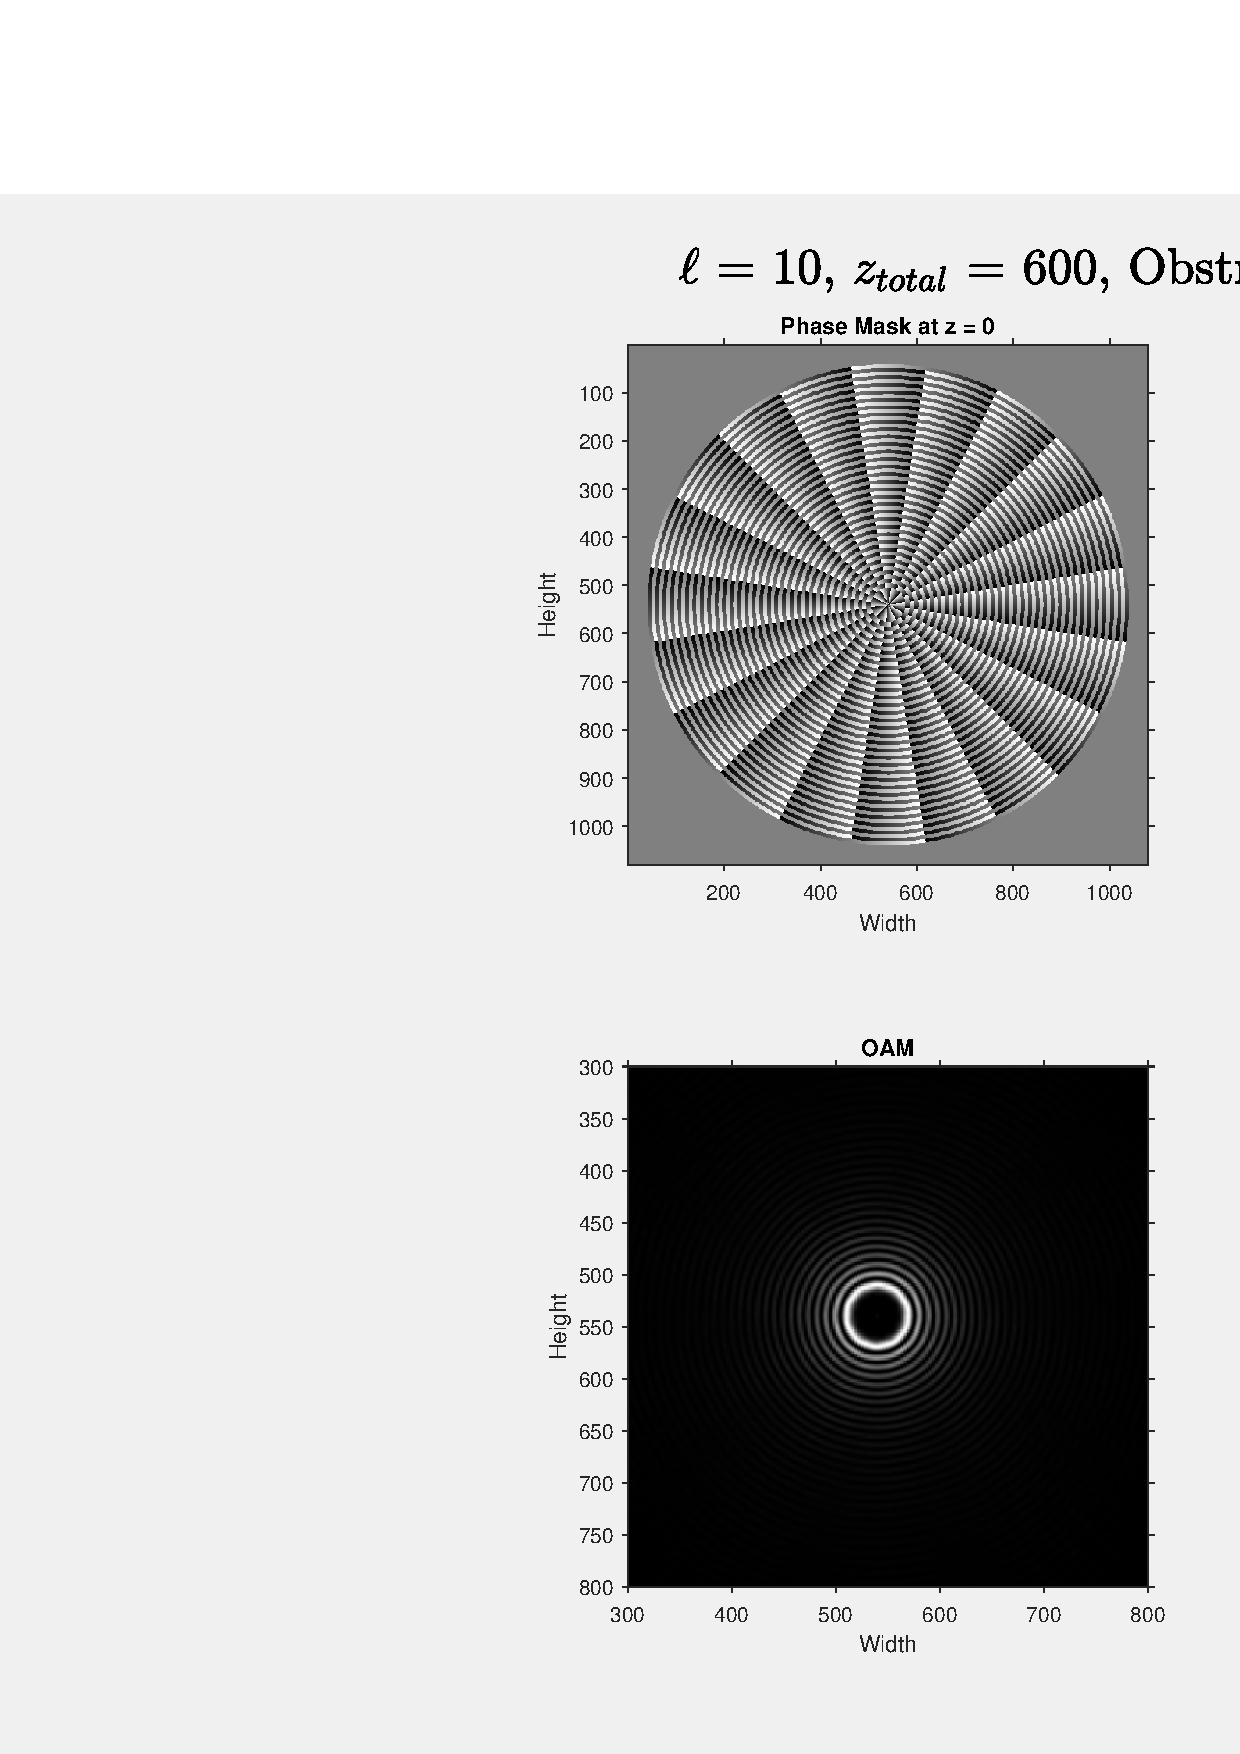
\includegraphics[width=\textwidth]{images/Appendices/Additional_Results/Rpx500_N60/type=1_r=0_zi=0_zf=600.png}
        \caption{$Rpx=500$ [px], $N = 60$ and $z = 600$.}
    \end{subfigure}
    \caption{Comparison between two unobstructed perfect vortices with different aperture and number of rings, propagated through different distances as well.}
    \label{fig:per_z=1000-vs-z=600}
\end{figure}

\begin{figure}[htbp]
    \centering
    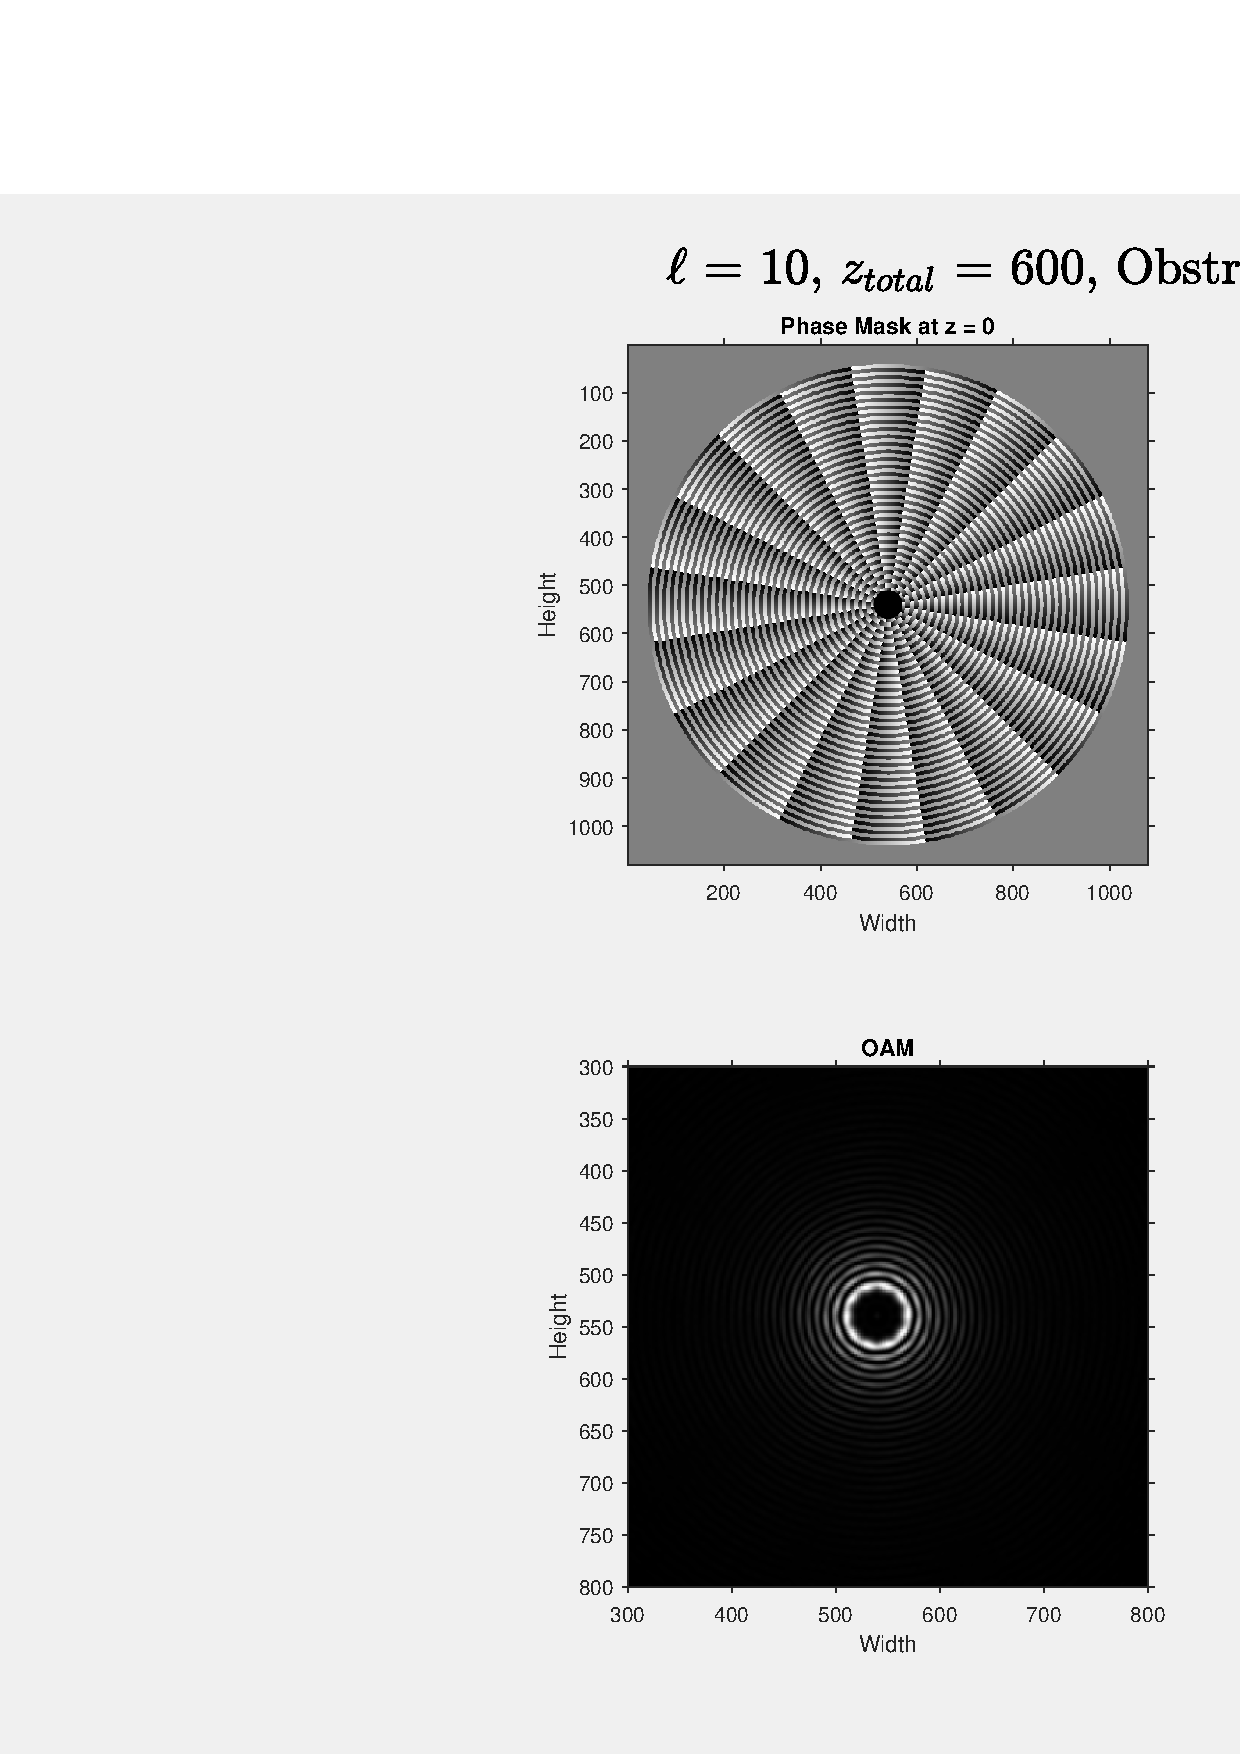
\includegraphics[width=12cm]{images/Appendices/Additional_Results/Rpx500_N60/type=1_r=30_zi=0_zf=600.png}
    \caption{Perfect vortex with $Rpx = 500$ [px], $N=60$, obstruction radius $r=30$ and propagated through $z = 600$ [mm].}
    \label{fig:new_perfect_r=30}
\end{figure}

\begin{figure}[htbp]
    \centering
    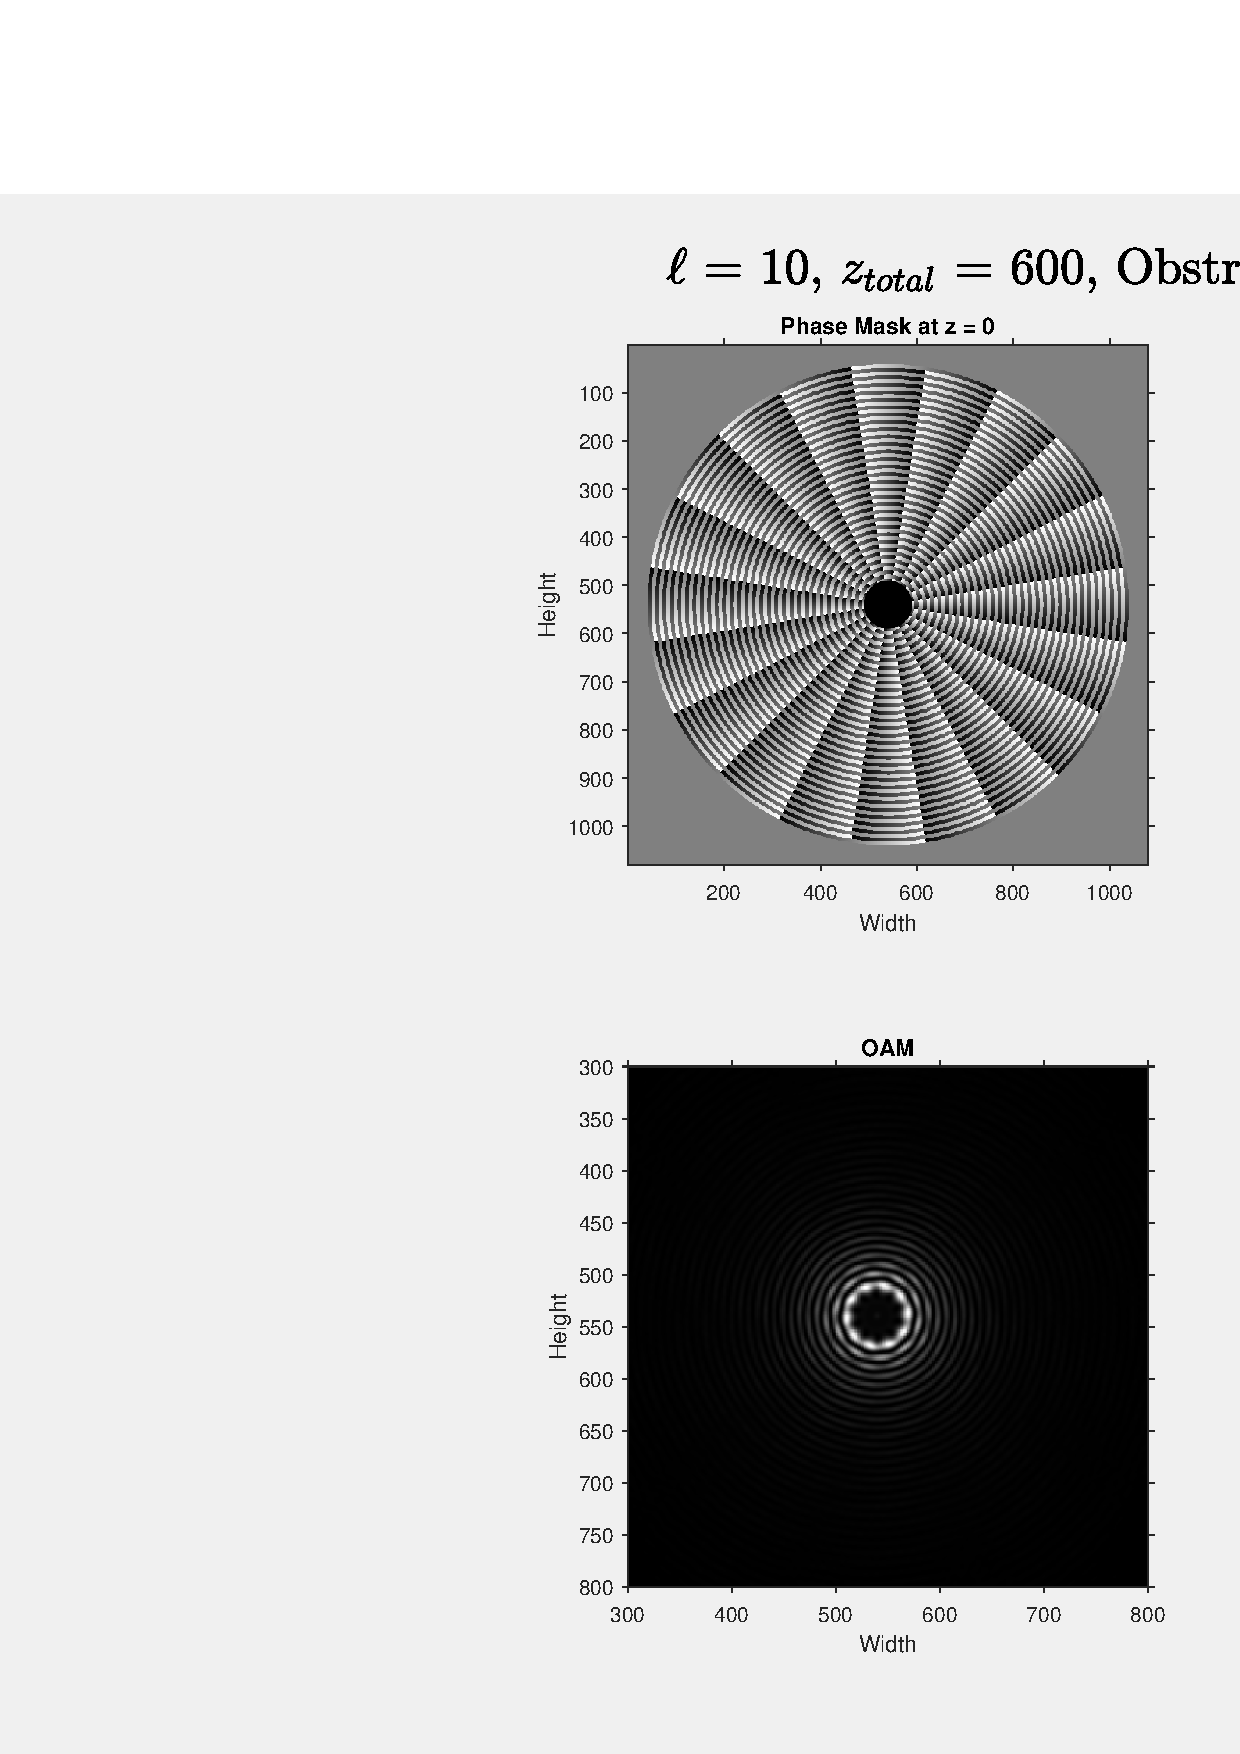
\includegraphics[width=12cm]{images/Appendices/Additional_Results/Rpx500_N60/type=1_r=50_zi=0_zf=600.png}
    \caption{Perfect vortex with $Rpx = 500$ [px], $N=60$, obstruction radius $r=50$ and propagated through $z = 600$ [mm].}
    \label{fig:new_perfect_r=50}
\end{figure}

\begin{figure}[htbp]
    \centering
    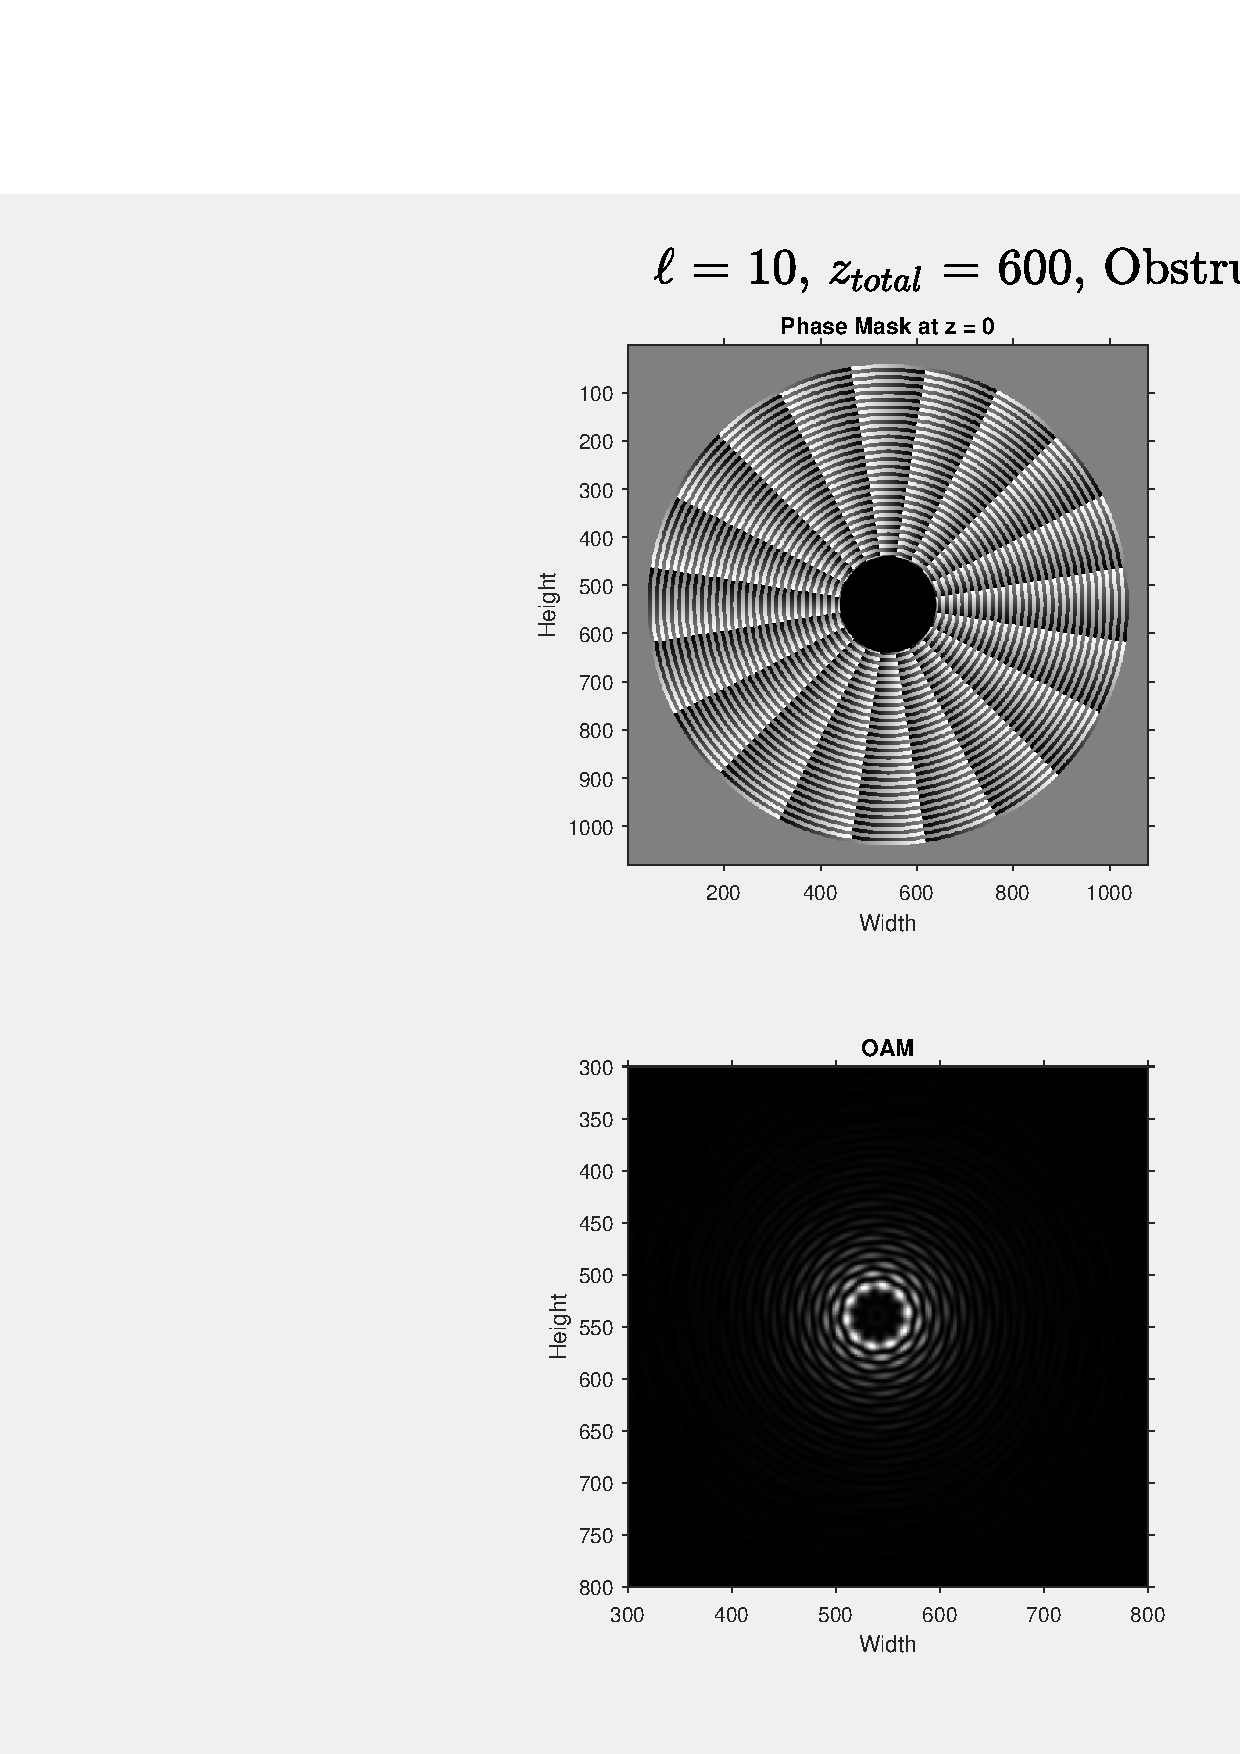
\includegraphics[width=12cm]{images/Appendices/Additional_Results/Rpx500_N60/type=1_r=100_zi=0_zf=600.png}
    \caption{Perfect vortex with $Rpx = 500$ [px], $N=60$, obstruction radius $r=100$ and propagated through $z = 600$ [mm].}
    \label{fig:new_perfect_r=100}
\end{figure}


\newpage
\section{Staged propagation results}

As it was stated in chapter \ref{Results}: Results, simulated propagation models are not perfect and can induce errors in the phase mask after each propagation. These errors are considerably amplified in staged propagation.

Staged propagation is a method implemented in this work to allow an unobstructed vortex to be propagated through a distance $z_i$, in [mm] until it encounters an obstruction of arbitrary size at that position. Then, the second stage of the propagation takes place, where the now-obstructed vortex is propagated through a distance $z_f - z_i$, also in [mm].

Now, the results presented in this section will not show the obstructed vortices, as in any other section or chapter. Instead, unobstructed staged propagations of $z_f = 1000$ [mm] and variable $z_i$ distances are shown, to highlight the destructive effect of this type of propagation. An alternative view of this is the following: if simulated staged propagation is true to reality, then unobstructed propagations should all look identical, since no scenario has more information than any other, in theory. In contrast, what is seen are completely different outcomes, which can only be explained by the cumulative errors introduced by the propagation models in a digital (or discrete) form.

\begin{figure}[htbp]
    \centering
    \begin{subfigure}[b]{0.45\textwidth}
        \centering
        \includegraphics[width=\textwidth]{images/Appendices/Additional_Results/Staged_Propagation/type=0_r=0_zi=100_zf=1000.png}
        \caption{Regular vortex.}
    \end{subfigure}
    \hfill
    \begin{subfigure}[b]{0.45\textwidth}
        \centering
        \includegraphics[width=\textwidth]{images/Appendices/Additional_Results/Staged_Propagation/type=1_r=0_zi=100_zf=1000.png}
        \caption{Perfect vortex.}
    \end{subfigure}
    \caption{Comparison between regular and perfect vortices on staged propagation with $z_i=100$ [mm].}
    \label{fig:staged_zi=100}
\end{figure}

\begin{figure}[htbp]
    \centering
    \begin{subfigure}[b]{0.45\textwidth}
        \centering
        \includegraphics[width=\textwidth]{images/Appendices/Additional_Results/Staged_Propagation/type=0_r=0_zi=200_zf=1000.png}
        \caption{Regular vortex.}
    \end{subfigure}
    \hfill
    \begin{subfigure}[b]{0.45\textwidth}
        \centering
        \includegraphics[width=\textwidth]{images/Appendices/Additional_Results/Staged_Propagation/type=1_r=0_zi=200_zf=1000.png}
        \caption{Perfect vortex.}
    \end{subfigure}
    \caption{Comparison between regular and perfect vortices on staged propagation with $z_i=200$ [mm].}
    \label{fig:staged_zi=200}
\end{figure}

\begin{figure}[htbp]
    \centering
    \begin{subfigure}[b]{0.45\textwidth}
        \centering
        \includegraphics[width=\textwidth]{images/Appendices/Additional_Results/Staged_Propagation/type=0_r=0_zi=500_zf=1000.png}
        \caption{Regular vortex.}
    \end{subfigure}
    \hfill
    \begin{subfigure}[b]{0.45\textwidth}
        \centering
        \includegraphics[width=\textwidth]{images/Appendices/Additional_Results/Staged_Propagation/type=1_r=0_zi=500_zf=1000.png}
        \caption{Perfect vortex.}
    \end{subfigure}
    \caption{Comparison between regular and perfect vortices on staged propagation with $z_i=500$ [mm].}
    \label{fig:staged_zi=500}
\end{figure}

Interestingly enough, perfect vortices also seem to show a better resistance to staged propagation, compared to regular ones. This only reassures the observations made in chapter \ref{Results} that perfect vortices are more resistant in general, and its responsibility can probably be pinpointed to its phase field, or phase mask. Regardless, at $z_i=500$ the vortex becomes distorted to the point that it is no longer an OAM: its rings are erratic and so is the central region, that was supposed to be dark.

To minimize this type of error in a simulation, then phase cleaning should be applied after each propagation, direct or staged, as it was also stated in section (\ref{c4:other arguments variations}).

To summarize the results of this particular section, if staged propagation can distort the vortex itself without the ``need'' of a central obstruction, like the ones studied in this paper, then adding the central obstruction will only further destroy the vortices that are already erratic.
